% REQUIREMENT ANALYSIS
\chapter{Requirement analysis}\label{chapter:requirement_analysis}

\section{User story and storyboard}\label{section:story}

The use of the application can be illustrated by the following  user story. Figure \ref{figure:storyboard} depicts the same story line.

\begin{figure}
	
\includegraphics[width=200px]{img/filename}
	\caption{Story board depicting a potential scenario of use.}
	\label{figure:storyboard}
\end{figure}


%%%%%%%%%% USER STORY
\textit{Jake is a student at the department of computer science at KULeuven. For his project of Multimedia he has to develop an Android application. Unfortunately he has encountered a particular problem as he was working on the application. He decides to look for some help.}

\textit{He starts the application and enters his question. He also attaches a number of specialities as tags to his post. Users that are listed as specialists in these technologies are then notified and can start working on a solution.}

\textit{Several solutions are proposed. Jake finds one that works and is able to continue with his work.}


% tag system ---> hierarchical (but more specific tags may have multiple parents)

% open (still open for discussion) and closed questions
% public (visible for everyone) / private
% open forum (everyone can participate), closed forum

% the recipient of a question, can suggest other question recipients, or delegate the question

% chatbox available, but can be turned off, or made available for groups of people
% (if necessary only during selected periods of time, e.g. personalized help)
% tutors can get a licence to teach, private students can pay money for private lessons
% (in contrast to public lessons / questions)

% !!! "interests" :
%	person 1 :  I would like to learn skill X
%	person 2 : I would like to learn skill Y
%	person 3 : I am good at skill X
%	person 4 : I would like to help people with skill Y
%		SUGGESTION system :
%		person 1 and person 4 are matched
%		person 2 and person 3 can be matched as well... (e.g. to person 3: person 2 would like to learn a skill you are good at, care to help him/her?) How did you started learning this skill? ...


\section{Use case diagram}\label{section:usecase}

The use case diagram for the application is shown in  figure \ref{figure:use_case_diagram}. Each use case is elaborated in tables \ref{table:use_case1}, \ref{table:use_case2} and \ref{table:use_case3}.

\begin{figure}
	\begin{center}
		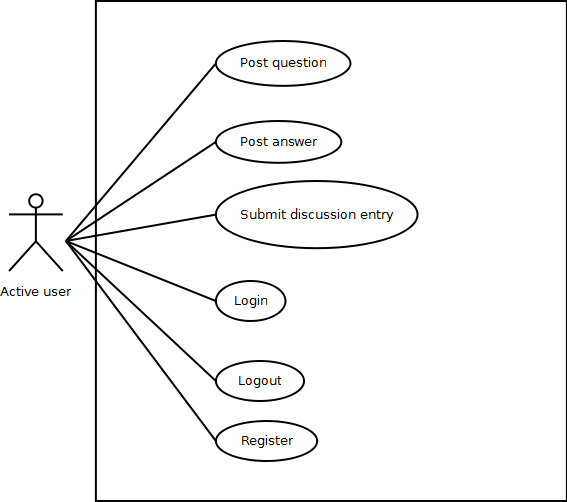
\includegraphics[width=200px]{img/use_case_diagram}
	\end{center}
	\caption{The use case diagram showing the functionality in the system from a user's perspective.}
	\label{figure:use_case_diagram}
\end{figure}


\begin{table}[h]
\caption{Use case 1 \textit{Post question}}
\begin{center}
	\begin{tabular}{ l p{300px} }
		\hline
		\textbf{Primary actor:}	& Active user \\

		\textbf{Preconditions:}	& User is logged in; \\

		\textbf{Basic flow:}	& (1) The question form is loaded. \\
													& (2) The user enters his question. \\
													& (3) The user selects recipients, including specific people and groups. \\
													& (4) The user submits the form data. \\
													& (5) The systems shows a confirmation message. \\

		\hline
	\end{tabular}
\end{center}
\label{table:use_case1}
\end{table}


\begin{table}[h]
\caption{Use case 2 \textit{Post answer}}
\begin{center}
	\begin{tabular}{ l p{300px} }
		\hline
		\textbf{Primary actor:}	& Active user \\

		\textbf{Preconditions:}	& User is logged in; \\
														& The user has selected a question to answer. \\
														& User is allowed to participate in the discussion. \\

		\textbf{Basic flow:}	& (1) The user selects an option to answer the question. \\
													& (2) The user enters his/her answer. \\
													& (3) The user submits the answer. \\
													& (4) The systems shows a confirmation message. \\

		\hline
	\end{tabular}
\end{center}
\label{table:use_case2}
\end{table}



\begin{table}[h]
\caption{Use case 3 \textit{Take part in discussion.}}
\begin{center}
	\begin{tabular}{ l p{300px} }
		\hline
		\textbf{Primary actor:}	& Active user \\

		\textbf{Preconditions:}	& The user is logged in; \\
														& The user has found a question he/she would like to provide further comments on; \\
														& The user is allowed to participate in the discussion.\\

		\textbf{Basic flow:}	& (1) The user selects an option to create a discussion entry. \\
													&	(2) The user types in the discussion entry.	\\
													& (3) The user submits the entry. \\
													& (4) The entry is added to the discussion. \\

		\hline
	\end{tabular}
\end{center}
\label{table:use_case3}
\end{table}



\section{Screen transition diagram}\label{section:screen_transitions}


\begin{figure}
	\begin{center}
		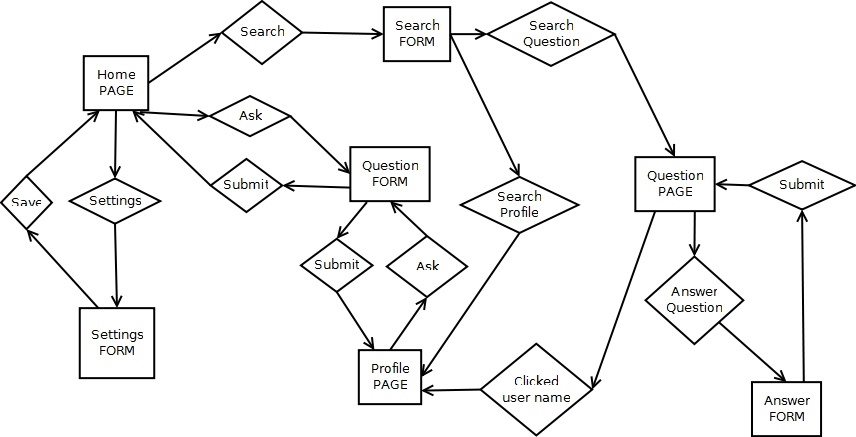
\includegraphics[width=400px]{img/screen_transition_diagram}
	\end{center}
	\caption{The transitions between the screens.}
	\label{figure:screen_transition_diagram}
\end{figure}





\section{Summary}

The following tries to summarize some of the requirements to support previously described functionality:

\begin{itemize}
	\item Users have to be able to interact with each other via the app on their device;
	\item	Users can be identified through a unique set of credentials;
	\item Users have to be able to post questions and answers in text format, or if possible, other types of multimedia;
	\item Data is persisted across sessions;
	\item	Users receive updates when new data is available, or alternatively can request for updates to be downloaded, e.g. by refreshing the page;
\end{itemize}


